%%%%%%%%%%%%%%%%%%%%%%%%%%%%%%%%%%%%%%%%%
% Lab Book 
% Original author:
% Frank Kuster (http://www.ctan.org/tex-archive/macros/latex/contrib/labbook/)
%
% Important note:
% This template requires the labbook.cls file to be in the same directory as the
% .tex file. The labbook.cls file provides the necessary structure to create the
% lab book.
%
%
% HOW TO USE THIS TEMPLATE 
% Each day in the lab consists of three main things:
%
% 1. LABDAY: The first thing to put is the \labday{} command with a date in 
% curly brackets, this will make a new page and put the date in big letters 
% at the top.
%
%%%%%%%%%%%%%%%%%%%%%%%%%%%%%%%%%%%%%%%%%

%----------------------------------------------------------------------------------------
%	PACKAGES AND OTHER DOCUMENT CONFIGURATIONS
%----------------------------------------------------------------------------------------

\documentclass[idxtotoc,hyperref,openany]{labbook} % 'openany' here removes the gap page between days, erase it to restore this gap; 'oneside' can also be added to remove the shift that odd pages have to the right for easier reading

\usepackage[ 
  backref=page,
  pdfpagelabels=true,
  plainpages=false,
  colorlinks=true,
  bookmarks=true,
  pdfview=FitB]{hyperref} % Required for the hyperlinks within the PDF
  
\usepackage{booktabs} % Required for the top and bottom rules in the table
\usepackage{float} % Required for specifying the exact location of a figure or table
\usepackage{graphicx} % Required for including images
\usepackage[parfill]{parskip}
\usepackage{amsmath}
\usepackage{amssymb}
\usepackage{csquotes}
\graphicspath{{./images/}}

\newlength{\mylen}
\setbox1=\hbox{$\bullet$}\setbox2=\hbox{\tiny$\bullet$}
\setlength{\mylen}{\dimexpr0.5\ht1-0.5\ht2}
\renewcommand\labelitemi{\raisebox{\mylen}{\tiny$\bullet$}}

\newcommand{\HRule}{\rule{\linewidth}{0.5mm}} % Command to make the lines in the title page
\setlength\parindent{0pt} % Removes all indentation from paragraphs

\DeclareMathOperator*{\argmax}{arg\,max}

%----------------------------------------------------------------------------------------
%	DEFINITION OF EXPERIMENTS
%----------------------------------------------------------------------------------------

%\newexperiment{shorthand}{Description of the experiment}

%---------------------------------------------------------------------------------------

\begin{document}

%----------------------------------------------------------------------------------------
%	TITLE PAGE
%----------------------------------------------------------------------------------------

\frontmatter % Use Roman numerals for page numbers
\title{
\begin{center}
\HRule \\[0.4cm]
{\Huge \bfseries Research Journal}\\
\HRule \\[1.5cm]
\end{center}
}
\author{\Huge Jerome Wynne \\ \\ \LARGE University of Bristol \\[2cm]}
\date{19th June 2017 - Present}
\maketitle

\tableofcontents

\mainmatter

%----------------------------------------------------------------------------------------
%	LAB BOOK CONTENTS
%----------------------------------------------------------------------------------------

% Blank template to use for new days:

%\labday{Day, Date Month Year}

%\experiment{}

%Text

%-----------------------------------------

%\experiment{}

%Text

%----------------------------------------------------------------------------------------

\labday{Thursday, 1st June 2017}
\experiment{Summary}
\begin{itemize}
	\item Set up this labbook.
	\item Wrote down what I'd like to achieve during my placement.
	\item Listed a bunch of classic \emph{Computer Vision} papers.
\end{itemize}

\experiment{Placement objectives}
During my 8-week placement I would like to:
\begin{itemize}
	\item Apply and understand the most useful \emph{Computer Vision} algorithms.
	\item Write either a statistics, machine learning, or \emph{Computer Vision} research paper worthy of publication.
	\item Develop a systematic workflow to problems involving data, and demonstrate this workflow in publicly available scripts or notebooks.
\end{itemize}

\experiment{Reading a paper critically}
\begin{itemize}
\item Motivations for the problem posed
\item The choices made in finding a solution
\item The assumptions behind the solution
\item The validity of those assumptions
\item Whether assumptions can be removed without invalidating the approach
\item What was accomplished
\item Future research directions
\end{itemize}
\newpage

\experiment{Structuring your time}
I think it's realistic to aim for 12 hours of productive work each day. This includes reading, studying, and running my own experiments. To begin with, I think I should spend at least three-quarters of this time learning. Maybe by week four I will shift the ratio.

 I will see how it goes, but I suspect I will prefer to work from the University rather than DNV-GL's offices.
 
 To make this placement a success, I will need to be disciplined about how I use my time. I know that if I get up early and immediately go to work, I can easily crack out four hours without breaking a sweat. After this time I can take at least a couple of hours - go to the gym, read, walk, or - of course - eat. After that I'll get back on that horse for another four or five hours, before taking another short break, then do a few more hours.
 
 Having lots of sleep is important for my mental health and emotional wellbeing, so I should aim to get at least eight hours. If I get up at six, this means that I should go to bed at half-nine. I can work from my flat, University buildings, or the DNV-GL offices. It would be a good idea to mix the places I study up - I know this has helped me keep focused in the past. I need to be careful to provide some time for myself too, so that I can recuperate: I think two hours at the end of the day, eight until ten, will be enough.
 
 \experiment{Figuring out what to write about}
 \begin{enumerate}
 \item Narrow down your field of study
 \item Define what to investigate
 \item Establish a thesis or an argument
 \end{enumerate}

I am studying \emph{Computer Vision} and statistics. This is because I want to build robust algorithms to understand visual information, which in turns makes it easier to automate difficult or tedious tasks, such as watching CCTV cameras or spotting damage to structures in video footage. I am doing this so that we will know more about how patterns in visual information can be found, and so that we can exploit these patterns to automate economically and socially beneficial tasks. I am also interested in how we can represent visual information to make it easier to work with and to understand.

\experiment{Structuring your work}
\begin{enumerate}
\item Find data that poses an unsolved problem, or find a problem that needs data to be solved.
\item Find the data, or pose the problem.
\item Review the relevant literature.
\item Propose a solution, then run experiments and conduct analysis to test that solution.
\item Write up the results.
\end{enumerate}

\experiment{How to use this book}
I should use this book to record what I'm doing, ideas and conversations I have, experiments I run, papers and books to read, things I understand and don't understand - everything related to my research. It only takes a few minutes to put a screenshot in this document - remember this!

As a habit, at the beginning of each day I will write down what I plan to do. At the end of the day I'll review what I've done. I should also review the book each week, to get an idea what I've been up to and where I'm headed.

\newpage
%-----------------------------------------------
 % 		PAPERS
 %---------------------------------------------
{\hspace{5cm} \Huge\textbf{Papers} \hfill}
\\

\begin{table}[h!]
\hspace{-2.5cm}
\centering
\renewcommand{\arraystretch}{1.5}
 \small
\begin{tabular}{@{}p{6cm} p{4cm} p{1cm} p{3cm} p{1cm}} \toprule
\textbf{Title}		&	\textbf{Authors}	&	\textbf{Year}		&	\textbf{Topic}		& 	\textbf{Read}\\ \midrule
Theory of Edge Detection	&	D. Marr, E. Hildreth	&	1980	&	Computer vision	& No \\
A Computational Approach to Edge Detection & J. Canny & 1986 & \emph{Computer Vision} & No \\
Determining optical flow	&	B.K.P. Horn, B. Schunk	&	1981	&	Computer vision	&	No \\
An iterative image registration technique with an application to stereo vision	&	B. Lucas, T. Kanade	& 1981 &	Computer vision	&	No \\
Snakes: Active contour models	&	M. Kass, A. Witkin, D. Terzpoulos	&	1988 & \emph{Computer Vision} & No \\
Eigenfaces for recognition & M. Turk, A. Pentland & 1991 & \emph{Computer Vision} & No \\
Shape and motion from image streams under orthography: a factorization method & C. Tomasi, T. Kanade & 1992 & \emph{Computer Vision} & No \\
Texture features for browsing and retrieval of image data & B. Manjunath, W. Ma & 1996 & \emph{Computer Vision} & No\\
Conditional density propagation for visual tracking & M. Isard, A. Blake & 1998 & \emph{Computer Vision} & No \\
Normalized cuts & J. Shi, J. Malik & 2000 & \emph{Computer Vision} & No \\
Non-parametric model for background subtraction & A. Elgammal, D. Harwood, L. Davis & 2000 & \emph{Computer Vision} & No\\
Distinctive image features from scale-invariant keypoints & D. Lowe & 2004 & \emph{Computer Vision} & No
 \\ \bottomrule
\end{tabular}
\end{table}


\labday{Monday, 19th June 2017}
\experiment{Summary}
\begin{itemize}
\item Arrived at DNV offices @ 10:00.
\item H \& S induction. Remember to look at the green lights above the doors!
\item Met Elizabeth Traiger:
\begin{itemize}
\item Solar panel cracks toy problem.
\item DNV are keen to use Python.
\item Approx. 1500 minutes of turbine data available.
\item We need a method for labeling the data.
\end{itemize} 
\item IT was not set up - she will email me tomorrow when it is ready.
\item DNV use Microsoft Azure services internally.
\item The company is open to using TensorFlow.
\item We agreed that weekly meetings would be appropriate. She is away this Friday (in London, speaking about using satellite imagery of windfarms to monitor fish populations (?), in association with the European Space Agency) and next week (site visit?).
\item Various ideas came up in our conversation: super-resolution methods, using simulation data, creating synthetic data, thinking about how to segment the images.
\item Footage from two turbines is available this week. More footage will be available next week.
\item I can VPN into DNV's network using the laptop that they provided me.
\item I left the DNV offices after lunch (14:00), then worked on the Design Project briefs until 16:30.
\item Liz planned to book a meeting with the inspections team to discuss how they look for damage. Possible questions:
\begin{itemize}
	\item What does damage look like?
	\item Over what time periods does it develop?
	\item What causes the damage?
	\item What mistakes do you make when looking for damage?
	\item What type of damage is easiest/most difficult to spot?
	\item What do you do when you find damage?
	\item What problems do you think there are with using drones to identify damage?
\end{itemize}
\end{itemize}

In the afternoon I read the introduction to Canny's paper on edge detection. I learnt that there is a tension between edge detection and localization (the distance between the detected edge and the true edge). Apparently the paper determines the optimal operator for various common edges.

I also read the introduction and first chapter of S.J. Prince's book on computer vision. The introduction outlined the book's structure and the first chapter was a quick review of basic probability theory.

\begin{itemize}
\item Read Canny paper.
\item Read the Chapter 1, 3, and 6 of S.J. Computer Vision. Make notes and complete the associated exercises.
\item Apply what was learnt in this chapter using Python.
\item Outline the structure of compute vision / machine learning.
\end{itemize}

\experiment{Prince: \emph{Computer Vision} (Ch. 1, Introduction)}
The book's structure was outlined. It consists of six sections:
\begin{enumerate}
\item Probability.
\item Machine learning for machine vision.
\item Graphical models (principled ways to simplify the relationship between image data and estimated properties) for machine vision.
\item Image preprocessing.
\item Geometric machine vision - generating 3D models based on image data and localizing a camera based on its view.
\item Families of machine vision models for common problems.
\end{enumerate}
It took me about ten minutes to read through this first chapter of five pages. Relevant papers are listed at the end of each of the book's sections.

\experiment{Prince: \emph{Computer Vision} (Ch. 2, Introduction to Probability)}
The second chapter took about an hour to read and make notes for. Almost all of it was review material: random variables, distributions, joint distributions, Bayes' rule, conditionality, and expectation. I did learn, however, two useful things:
\begin{itemize}
\item A Hinton diagram can be used to visualize probability mass functions. A square is associated with each point; the square's area relative to the total area of all squares corresponds to that value's relative probability. Figure \ref{fig:hinton_diagram} shows a Hinton diagram in two variables.
\begin{figure}[h!]
\centering
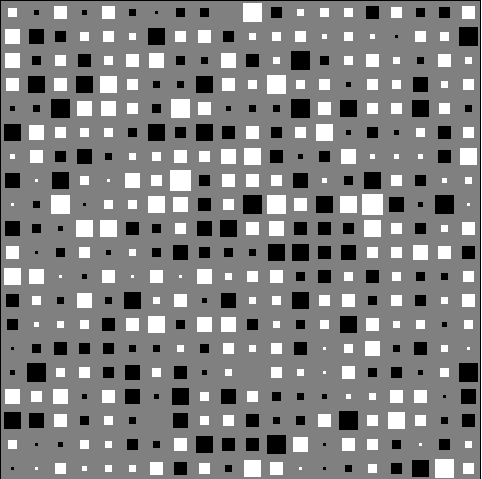
\includegraphics[width=0.5\textwidth]{hinton_diagram.png}
\caption{A Hinton diagram can be used to visualize probability mass functions in one or two variables.}
\label{fig:hinton_diagram}
\end{figure}
\item A useful identity: if two random variables are independent, then the product of their expectation is equivalent to the expectation of their product. More generally:
\begin{equation}
	E[f(x) \cdot g(y)] = E[f(x)] \cdot E[g(y)]
\end{equation}
\end{itemize}



\labday{Tuesday, 20th June 2017}
\experiment{Summary}
I woke at six (I'm getting the hang of it). For the first hour of the day I reviewed the project brief MZ had commented on and sent it off to PH. PH mentioned I could use his office for the next two weeks while he was away - hopefully I can pick up the key from him this afternoon.

Today I would like to complete Chapters 3 and 4 of Prince's Computer Vision, do some modeling in Python, and begin the CVX course. I should also get an overview of the main \emph{Computer Vision} tools for Python.

I made notes on Chapter 3 and completed five of its exercises, which related to conjugacy, the exponential family, and the modes of the distributions studied. PH said to pick up the key to his office from the porter. ET emailed me to say that IT have set up my account - I agreed to go in tomorrow morning to meet her and pick up my laptop. I should also ask her when we plan to meet the wind turbine inspections team.

I intend to complete Chapter 4 this afternoon. I am now going to read Canny's paper.
I tried to read Canny's paper but kept zoning out. I did understand, however, that he formulated an optimization problem by expressing detection performance as signal-to-noise ratio and localization performance as a similar quantity but involving gradients.

I spent fifty minutes reading through Chapter 4. I made notes on maximum likelihood, maximum a posteriori, and bayesian methods for optimizing parameter estimates. I read through an example wherein the mean and variance of a univariate normal distribution were estimated using a normal-scaled inverse gamma prior; as it turns out, the benefits of using the conjugate here are twofold - not only does the posterior have a closed-form solution, but so also does the posterior predictive!

\experiment{Prince: \emph{Computer Vision} (Ch. 3, Common Probability Distributions)}

I started on Chapter 3 of Prince's book yesterday. It covers eight probability distributions that will be useful for machine vision purposes. Four of these are for modelling image data or world properties; the other four are for modelling the parameters of these four. I made notes, but have yet to complete the exercises. The distribution pairs covered were:
\begin{itemize}
	\item Bernoulli - Beta
	\item Categorical - Dirichlet
	\item Univariate normal - Normal-scaled inverse gamma
	\item Multivariate normal - Normal inverse Wishart
\end{itemize}
The four distributions on the left were familiar to me, as was the beta distribution (however it was useful to note that the expectation of $\text{Beta}[\alpha, \beta]$ is defined by $\frac{\alpha}{\alpha + \beta}$). The Dirichlet, normal-inverse scaled gamma, and normal inverse wishart distributions were new to me. 

The Dirichlet distribution is effectively a generalization of the beta distribution to cover more than one variable. It's used to model the $K$ parameters of a categorical distribution. As such, $\sum_k \lambda_k = 1$ at all points in the Dirichlet distribution. Its hyperparameters $\alpha_1, ..., \alpha_K$ describe the categorical distribution's expecations over each of its variables $E[\lambda_1], ..., E[\lambda_K]$; the magnitude of the $\alpha$ values determines the Dirichlet's dispersion.

The Normal-scaled inverse gamma distribution is used to model uncertainty in the mean and variance of a univariate normal distribution. It has four parameters. In a similar vein, the normal inverse Wishart distribution describes uncertainty in the mean vector and covariance matrix of a multivariate normal distribution.

I'm now going to complete three questions from the exercises, then go to the barbers. When I get back I will complete three more exercises, before continuing to read the Canny paper.

I completed three questions. The first asked for the mode of the beta distribution (found by maximizing the pdf w.r.t. the variable). The second pointed out that all of the distributions in the chapter were members of the exponential family; it then requested the beta pdf in exponential family form. The third related a normal prior and restricted normal likelihood to a normal posterior (i.e. it was a conjugacy problem). These questions together took me about forty-five minutes to complete.

This is not the first time the exponential distribution has been mentioned - why is understanding multiple distributions as variants on one distribution useful?

I completed two more questions: showing that the normal-scaled inverse gamma is the conjugate prior to the univariate normal distribution; showing that the Dirichlet distribution is the conjugate prior to the categorical distribution. They were mostly exercises in algebra, but it did drive home why the Dirichlet and normal-scaled inverse gamma distributions are relevant, and what they look like (particularly w.r.t. the Dirichlet-beta similarities).

\experiment{Prince: \emph{Computer Vision} (Ch. 4, Fitting Probability Models)}
The chapter began with maximum likelihood, maximum a posteriori, and bayesian methods for optimizing parameter estimates. I read through an example in which the mean and variance of a univariate normal distribution were estimated using a normal-scaled inverse gamma prior; as it turns out, the benefits of using the conjugate here are twofold - not only does the posterior have a closed-form solution, but so also does the posterior predictive! I think I would benefit from writing out the Bayesian solution, and possibly running a simulation in Python. Maybe I'll go through the other example before building the simulation.

I made notes on both worked examples. The second example involved inferring posterior and posterior predictive distributions from a categorical likelihood and its conjugate (a Dirichlet prior). As in the case of the univariate normal - normal-scaled inverse gamma problem, bott distributions had neat solutions. The posterior was another Dirichlet distribution (with correspondingly updated parameters $\tilde{\alpha}_j = \alpha_j + N_j$) and the posterior predictive turned out to be a function of beta functions.

I'm going to write two R simulations, one for each example.

I built an R simulation for the first example.

I attempted Q4.6, but fell short (the algebra became untangled). I will try again tomorrow morning; perhaps doing Q4.5 first will make it slightly easier. Once I've done those two questions, I should like to do Q4.7-4.10.
Worked 4 - 7:30 on Com. Vis. Chapter 4.

This evening I watched the first lecture from the CVX course. It explained what convex optimisation is, common variants of it (least squares and linear programming), discussed application areas, defined a convex functoin, provided an overview of the course, and gave some history on the topic.




\labday{Wednesday, 21st June 2017}
\experiment{Summary}
Today I plan to:
\begin{itemize}
	\item Complete the exercises from Ch. 4 of Computer Vision
	\item Walk through one of the examples available at PyImageSearch
	\item Read Ch. 5 of \emph{Computer Vision} and complete the associated exercises
	\item Pick up Paul Harper's office key
	\item Meet ET at 10:00 to have IT induction
	\item Explore solar panel dataset
	\item Investigate Python tools for tagging images
	\item Read Chapter 1 of Boyd's Convex Optimisation
\end{itemize}

(07:00 - 09:50) 
I spent the first hour and forty-five minutes of the day completing Exercises 4.5 - 4.10 of Computer Vision. I then made notes on Chapter 5, which is focused on the normal distribution. It began by showing the difference between spherical, diagonal, and full covariance matrices - spherical matrices have circular isodensity contours, diagonals have ellipsoidal ones whose axes are aligned with coordinate axes, and full covariance matrices have ellipsoidal contours in any orientation.

As it happens, it's possible to rotate a distribution's coordinate system to permit a full covariance matrix to be reexpressed as a diagonal one. The rotation matrix is deduced using the singular value decomposition (something I should probably know, but don't). I'm about to head off to DNV, but I intend to watch Gilbert Strang's lecture on the singular value decomposition when I get back. I think I could also do with inspecting matrix inverses more closely.

I spent the afternoon (10:30 - 16:00) in the DNV offices getting set-up with IT and so on. I also went through the two datasets made available to me so far. In the evening I wrote a Python script to resize and subset the PV panel images. I also skimmed Ch. 6 of Computer Vision.

Tomorrow morning I should label a few hundred of these images and try out the algorithms described in Ch. 6 of Com. Vis. For the first three hours of the day I should like to study from the book. The middle hours can be spent labelling and coding, before returning again to studying. I will read through Ch. 1 of S. Boyd's book on convex optimization also.

I did find a tool for annotating images - it's called Fiji (https://fiji.sc/). I should really start time-stamping my entries on this...

I also read a paper [\emph{Detection and Classification of Surface Defects on Gun Barrels Using Computer Vision and Machine Learning}, Sanmuhamani et al.] on gun barrel damage classification. They had success using an extended maxima transform was used to segment their images. They used sequential forward-feature selection. The six features that presented themselves as most useful (in a texture-based classification problem, fed into a radial-basis SVM) were:
\begin{itemize}
	\item Mean
	\item Variance
	\item Smoothness
	\item Skewness
	\item Uniformity
	\item Entropy
\end{itemize}
I think it would be worthwhile getting the definitions for these should any texture-based classification work come up.

I need to start logging to-dos using the Office 365 Planner app.

\experiment{PV Panels}
The first dataset is a ~50 scans of PV panels. Possible objectives with these panels are:
\begin{itemize}
	\item Detecting cracks.
	\item Detecting pit marks.
	\item Detecting blown cells.
\end{itemize}
An example image is shown in Figure \ref{fig:example_pv_cell}. I made a repo for the PV project.

\begin{figure}
\centering
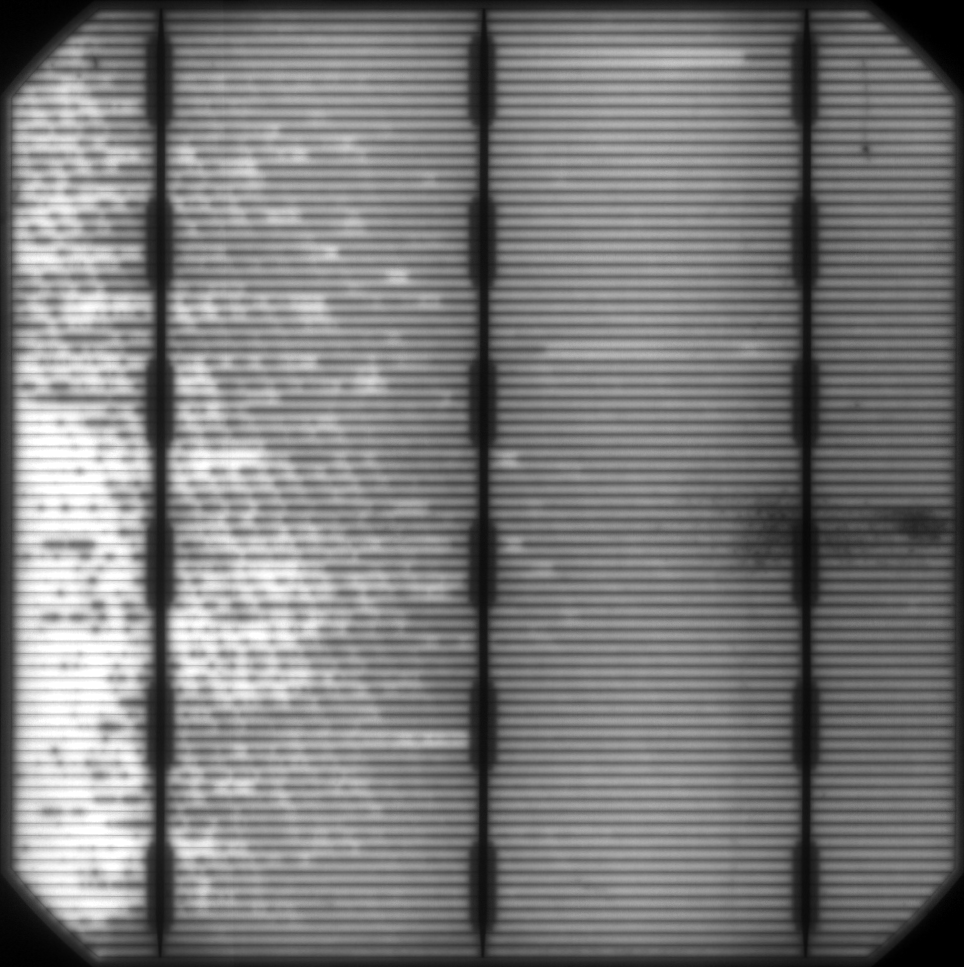
\includegraphics[width=0.5\textwidth]{pv_cell.png}
\caption{A sample image from the PV panels dataset.}
\label{fig:example_pv_cell}
\end{figure}

\experiment{PV Panels: Crack detection}
The objective of this task is to label images as according to whether or not they contain a crack - I don't think bounding boxes are appropriate. I'm going to begin by:
\begin{itemize}
	\item Rescaling the images to a constant size.
	\item Labeling the panels according to the damage they've incurred.
	\item Sorting the panels according to their type.
\end{itemize}

I created \texttt{panel-resizer.ipynb} to rescale the panel images to a fixed size\footnote{I deleted one duplicated image (52) and removed three smaller images}. This took me about an hour. While doing this, I realized that I could cluster the panels according to their metropolis distance from one another, generate an `undamaged' panel for each class, then use subtraction to identify damaged panels. I think the biggest weakness with such an approach, however, is the need for an `undamaged' panel image. How is easy would this be to generate synthetically?
\begin{enumerate}
	\item Label images (crack/no crack).
	\item 70/30 split of training/test data.
	\item Benchmark `dumb' classifiers.
	\item Select the best dumb classifier and optimize it.
\end{enumerate}


\labday{Thursday, 22nd June 2017}
\experiment{Summary}
Today I planned to:
\begin{itemize}
	\item Review what I covered yesterday.
	\item Read the blog post ``Classifying plankton with deep neural networks''.
	\item Label at least 50\% of the PV panel data.
	\item Set up a LaTeX report for the PV panel data.
	\item Update my current strategy for the PV data on Office 365.
	\item Complete problem exercises from Ch. 6 of \emph{Computer Vision}.
	\item Implement the algorithms presented in Ch. 6 of \emph{Computer Vision} on a dummy dataset.
	\item Benchmark 3 dumb classifiers against the labeled PV panel data.
	\item Read Ch. 1 of Boyd's \emph{Convex Optimisation}.
\end{itemize}
If there is time I will also begin reading Ch. 7 of \emph{Computer Vision}.

(07:30 - 08:00) I planned my approach to the PV panel crack detection task on Office 365.

(08:00 - 11:00) 

\experiment{PV Panels: Crack Detection}
To-dos:
\begin{itemize}
	\item Label subset images
	\item Build augmented images dataset
	\item Set up report
	\item Benchmark simple classifiers against augmented images
	\item Optimize best simple classifier
	\item Record simple classifier performances in report
	\item Set up Azure instance and train convnet against augmented images
	\item Upload augmented images dataset
	\item Investigate clustering of panels
\end{itemize}

\experiment{Prince: \emph{Computer Vision} (Ch. 5/6)}
Yesterday my work from this book constituted reviewing the many properties of the multivariate normal distribution, among which were:
\begin{itemize}
	\item The marginal distribution of a subset of a vector of normal r.v.s is also normal.
	\item The conditional distribution of a subset of vector of normal r.v.s, given the other r.v.'s values, is also a normal distribution.
	\item Its covariance matrix an be diagonalized using the singular value decomposition, which forms a rotation matrix that twists the reference frame to align with the axes of the distribution's ellipsoidal isodensity contours.
	\item It can have one of three types of covariance matrix - spherical, diagonal, or full - which determines how elliptical its isodensity contours are and what its orientation relative to the coordinate axes is.
\end{itemize}
In the evening I began work on Ch. 6, \emph{Learning and Inference in Vision}. It defined the basic task of machine vision as inferring world properties based on image data. It also outlined a framework for solving this problem consisting of three components:
\begin{itemize}
	\item A model relating image data to world properties.
	\item A learning algorithm for adjusting that model's parameters based on observations.
	\item An inference algorithm for returning a predicted world state based on input image data.
\end{itemize}
The model can be either discriminative or generative. A discriminative model describes $\text{Pr}(\mathbf{w}|\mathbf{x})$, the world state based on the image data. By contrast, a generative model instead represents the likelihood $\text{Pr}(\mathbf{x}|\mathbf{w}$) - what the image data should be for a given world state.

(08:20 - 9:20) Made notes on modeling a univariate continuous response with univariate continuous inputs using discriminative and generative methods. Also described how to model a binary response in terms of continuous image data, again via both generative and discriminative methods. 
 
\begin{itemize}
\item Univariate continuous data $x$, univariate continuous world state $w$
	\begin{itemize}
		\item Discriminative approach: Model $\text{Pr}(w|x)$ using $\text{Norm}_{w}[\phi_0 + \phi_1 x, \sigma^2]$. Fit $(\phi_0, \phi_1, \sigma^2)$ based on training set $\{x_i, w_i\}_{i = 1}^I$.
		\item Generative approach: Model $\text{Pr}(x|w)$ using $\text{Norm}_{x}[\phi_0 + \phi_1 w, \sigma^2]$, and $\text{Pr}(w)$  using $\text{Norm}_w [\mu_p, \sigma_p^2]$. Fit $(\mu_p, \sigma_p^2)$ using the available world states $\{w_i\}_{i = 1}^I$. Fit $(\phi_0, \phi_1, \sigma^2)$ using the training data $\{x_i, w_i\}_{i = 1}^I$. Compute the posterior using Bayes' rule. 
	\end{itemize}
\item Univariate continuous data $x$, binary world state $w$.
	\begin{itemize}
		\item Discriminative approach: Model $\text{Pr}(w|x)$ using a Bernoulli distribution parameterized by $\lambda = \text{sig}[\phi_0 + \phi_1 x] = \frac{1}{1 + \exp(-\phi_0 - \phi_1 x)}$. Fit $(\phi_0, \phi_1)$ using the training data.
		\item Generative approach: Set up a normal distribution over the data $\text{Pr}(x|w) = \text{Norm}_x[\phi_0 + \phi_1 w, \sigma^2]$ such that its parameters switch according to the world state $w \in \{0, 1\}$. Use a Bernoulli distribution for the world state prior $\text{Pr}(w) = \text{Bern}_w [\lambda_p]$ - fit $\lambda$ using the observed world states. For inference compute the posterior at the chosen set of inputs.
	\end{itemize}
\end{itemize}

(09:30 - 10:10) Read through skin detection and background subtraction examples and the chapter summary. The skin detection algorithm set up a generative model describing pixel intensity based on skin/non-skin status via a multivariate normal distribution. The prior was a Bernoulli distribution on the world states. By contrast, the background subtraction example set up a likelihood function wherein the pixel intensities of foreground objects were described using a uniform distribution (i.e. all combinations of $(x_R, x_G, x_B)$ were deemed equally likely) and the intensity at each background pixel  in each scene was expressed in terms of a multivariate normal distribution.

(10:20 - 11:45) Completed Ch.6 exercises 1, 3, 5, 7. Related modelling a continuous response against a binary world state to quadratic discriminant analysis and linear discriminant analysis (I ended up seeing this when comparing the for the decision boundary formed by two normal distributions with equiprobable associated classes with the decision boundary derived from a logistic regression classifier).

(12:50 - 13:45) Labeled PV panels dataset.

(14:00 - 16:05) Read (and made notes on) Ch. 7 of \emph{Computer Vision}.

(16:05 - 16:45) Typed up lab notes from this afternoon's work on hidden variables and the EM algorithm.

(19:15 - 22:15) Augmenting PV panel images. Image augmentations:
\begin{itemize}
	\item vertical flip
	\item rescaling
	\item adding noise
\end{itemize}

\experiment{Prince, \emph{Computer Vision} (Ch. 7, Modeling complex data densities)}

This chapter frames the methods introduced by considering the shortcomings of attempting to build a generative model for a face classifier. Given a worldstate corresponding to face/no face, $w \in \{0, 1\}$, what is the probability density function for each pixel's intensity in an image of a fixed size? We might choose to model this likelihood using a normal distribution whose parameters are fit using training data:
\[
	\text{Pr}(\mathbf{x}|w) = \text{Norm}_{\mathbf{x}}[\mathbf{\mu}, \mathbf{\Sigma}]
\]
Notice that given $w = 1$, the parameters will be $\{\mathbf{\mu}_1, \mathbf{\Sigma}_1\}$, and given $w = 0$ the parameters will be $\{\mathbf{\mu}_0, \mathbf{\Sigma}_1\}$. By defining a prior over the world state (a Bernoulli distribution whose parameter $\lambda$ is fit using training data), we can get a hold of a posterior describing the probable world state, given a particular image's set of pixel intensities, $\text{Pr}(w|\mathbf{x})$.

This modeling strategy has several shortcomings:
\begin{itemize}
	\item The normal distribution is sensitive to outliers - one extreme observation will set estimates of its mean and covariance way out of kilter.
	\item A unimodal distribution doesn't describe what pixel intensities are probable if someone's face is in an image - people have different skin, eye, and hair colours.
	\item An outrageous number of parameters needs to be estimated. Given a $30\times30$ RGB image, 2700 mean intensity values and $\frac{2700 \times 2701}{2}$ covariance values need to be estimated. To make this estimate unique then, about three-and-a-half million training examples are needed.
\end{itemize}
To get around these problems we can - respectively - use t-distributions, mixture models, and subspace models. All of these tools exploit hidden variables. A joint distribution over the variable being modeled $\mathbf{x}$ and a hidden variable $\mathbf{h}$ is defined such that when $\text{Pr}(\mathbf{x}, \mathbf{h})$ is marginalized over $\mathbf{h}$, a complex density function of $\mathbf{x}$ emerges. As with any distribution, this joint distribution is parameterized by some set of values $\mathbf{\theta}$ which are chosen to maximize the likelihood function:
\[
	\hat{\mathbf{\theta}} = \argmax_{\mathbf{\theta}} \Bigg[\sum_{i = 1}^I \log \Big[\int \text{Pr}(\mathbf{x}_i, \mathbf{h}_i | \mathbf{\theta})d\mathbf{h}_i\Big]\Bigg]
\]
The expectation maximization algorithm is used to maximize the likelihood. This algorithm proceeds by iteratively raising a lower bound on the likelihood function. The lower bound is a function of the parameters $\mathbf{\theta}$ and density distributions over the hidden variables. On the t\textsuperscript{th} iteration of the algorithm:
\begin{enumerate}
\item The boundary is raised as far as possible by setting the density functions $q_i(\mathbf{h}_i)$ to be $\text{Pr}(\mathbf{h}_i|\mathbf{x}_i, \mathbf{\theta}^[t-1])$.
\item $\mathbf{\theta}^{[t]}$ is chosen to maximize the log-likelihood for the given density functions. 
\end{enumerate}
The first step is called the E-step (for expectation) and the second step is called the M-step (for maximization). By executing this algorithm repeatedly, it is possible to converge upon a local maximum in the likelihood function (which may also be the global maximum).

 Use various scales of panel images to generate more data. 
 
 
 
 \labday{Friday, 23rd June 2017}
 
 (08:00 - 13:30) Read and made notes on Ch.7 of \emph{Computer Vision}. Covered hidden variables, expectation maximization, mixture of gaussians, the t-distribution, and factor analysis. Spent three hours building a mixture of gaussians model using World Happiness Report data. Figure \ref{fig:MoG} shows a fit being made with four component distributions. It may not look like much, but I learnt a lot from doing it!
\begin{figure}[h!]
\centering
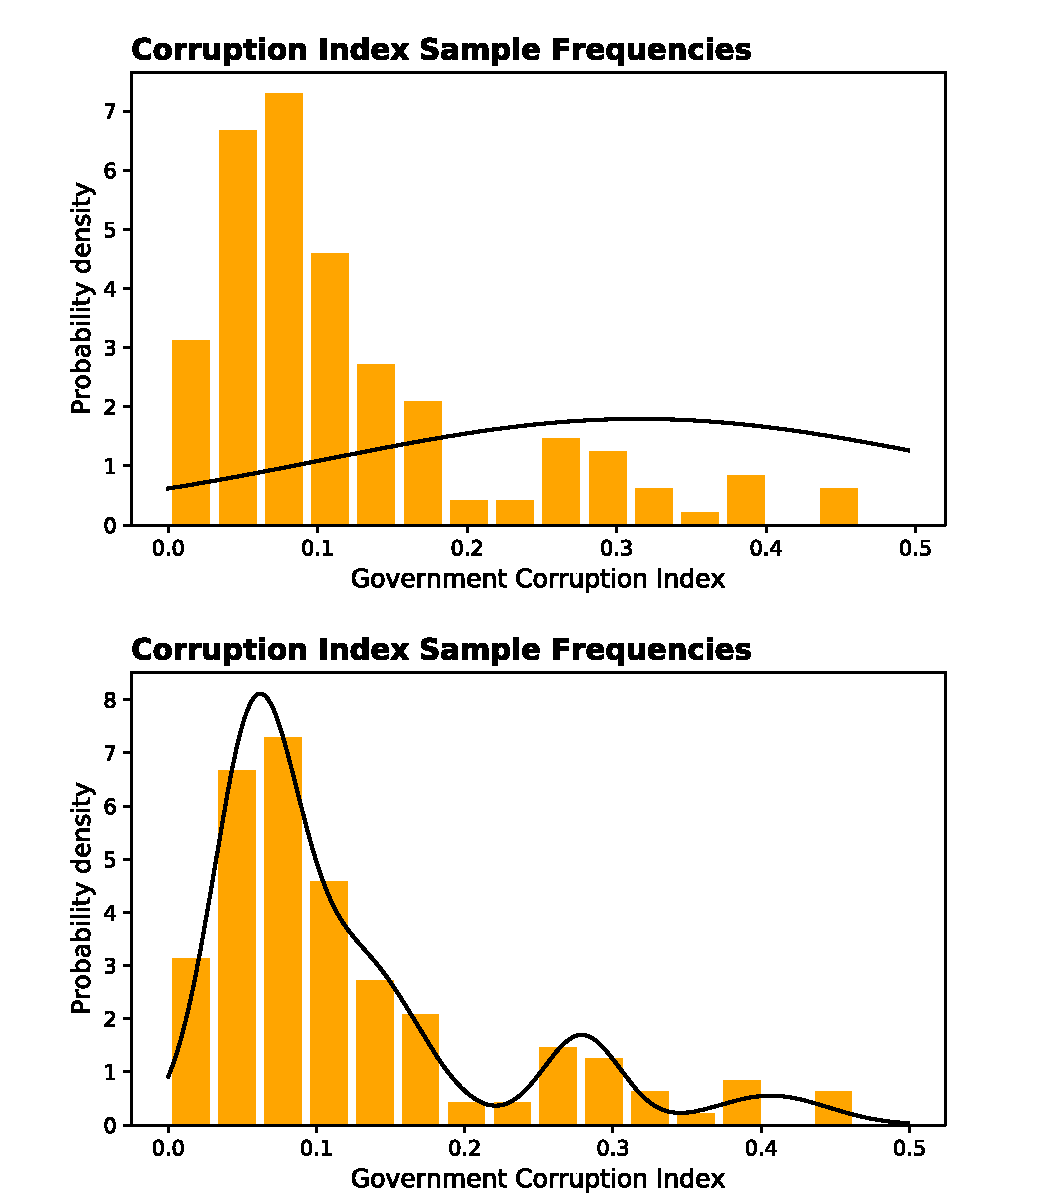
\includegraphics[width=0.7\textwidth]{MoG.pdf}
\caption{Fitting a four-component mixture of gaussians model using expectation maximization.}
\label{fig:MoG}
\end{figure}
 (16:00 - 17:45) Made notes on factor analyzers.
 
 (17:45 - 20:00) Ironed out some bugs in the PV panel organizer. Ran a random forest and an rbf SVM against augmented traiing data (they did all right, ~80\% accuracy). I'll type out what I did in more detail later.
 
 \experiment{Prince, \emph{Computer Vision} (Ch.7 Modeling Complex Data Densities)}
 So today I covered three things, all of in this chapter, all bearing a single commonality. They were introduced as tools with which to address weaknesses of using a normal model model for the likely intensities of a pixel (or some other continuous feature) for a given world state. In particular, a single peak probably doesn't represent reality very well, the parameter fits are very sensitive to outliers, and a vast number of parameters need to be determined as a result of the covariance matrix. The solutions to these problems, respectively, were:
 \begin{itemize}
 	\item Using a mixture of gaussians instead of one.
 	\item Using a t-distribution rather than a normal distribution.
 	\item Reducing the number of parameters to be determined by only modeling the covariation in directions where it is strongest.
 \end{itemize}
 Neatly, it turns out that all of these model variations can be represented in terms of hidden variables (which I described yesterday). A mixture of gaussians uses a categorically distributed hidden variable to weight the various normal distributions, each of which have their own covariance and mean. A variable with a t-distribution can actually be thought of as a normally distributed variable whose variance is parameterised by a scalar gamma-distributed variable. That is,
\begin{align*}
 	\text{Pr}(\mathbf{x}|\mathbf{h}) &= \text{Norm}_{\mathbf{x}_i}[\mathbf{\mu}, \mathbf{\Sigma}/h] \\
 	\text{Pr}(\mathbf{h}) &= \text{Gamma}_h[\nu/2, \nu/2]
\end{align*}
 While I had previously appreciated that the t-distribution's greater spread is a consequence of uncertainty w.r.t. its variance, this formulation made it especially clear what the role played by the degrees of freedom is.
 
 The third solution - factor analyzers - is something I'm still wrapping my head mathematically but I think I understand in principle. Sample a vector $\mathbf{h}$ from a multivariate standard normal distribution then use it to adjust the mean of a normal distribution to somewhere in the subspace described by its factors. Sample $\mathbf{x}$ from this shifted normal distribution. The hidden variable here is the sampled vector: the distribution of samples from the shifted normal distribution turns out to be normal also, but with a covariance such that:
 \[
 	\text{Pr}(\mathbf{x}|\mathbf{h}) = \text{Norm}_{\mathbf{x}_i}[\mathbf{\mu}, \mathbf{\phi\phi}^T + \mathbf{\Sigma}]
 \]
 Where $\mathbf{\phi}$ is a $D \times K$ matrix whose columns are the basis vectors (factors) of the subspace and $\mathbf{\Sigma}$ is a $D \times D$ diagonal (or spherical) covariance matrix. The factors are chosen to describe as much of the covariation in the full columnspace as possible, with the diagonal covariance matrix capturing the meat of the variance: a factor analyzer attempts to capture as much of the variation in the data's full $D$-dimensional columnspace in terms of an $\mathbb{R}^K$-dimensional subspace. One of the things I'm still trying to understand is why $\mathbf{\phi}\mathbf{\phi}^T$ represents covariation in the subspace - I plan to look at this today (I wrote the follow-up to the 23\textsuperscript{rd}'s work on the 24\textsuperscript{th}). As an aside, the author mentioned that when $\mathbf{\Sigma}$ is a spherical covariance matrix (that is, a scalar multiple of the identity matrix), this method is called principal component analysis. The benefit of using a spherical rather than a diagonal matrix is that it reduces further still the number of parameters to be fit (hence its widespread use when wrangling wide data).
 
 The reason the author framed the t-distribution, mixture of gaussian, and factor analysis model in terms of hidden variables is because density functions that can be expressed as a marginalization over a hidden variable (Equation \ref{eq:hidden_variable_marginalization}) lend themselves to optimization via expectation maximization.
 \[
 	\text{Pr}(\mathbf{x|\mathbf{\theta}}) = \int\text{Pr}(\mathbf{x}, \mathbf{h}|\mathbf{\theta})\cdot d\mathbf{h}\label{eq:hidden_variable_marginalization}
 \]
 The model parameters $\mathbf{\theta}$ can be fit by iterative maximization of a bound on the l.h.s's likelihood function. This bound is a function of the r.h.s.; EM raises this boundary by iteratively:
 \begin{itemize}
 \item updating density functions over the hidden variables,
 \item maximizing the boundary's value by adjusting the values of the parameters in $\mathbf{\theta}$.
 \end{itemize}
 Eventually, the boundary converges on the log-likelihood function such that a set of locally optimal parameter values are found.
 
 As I said, I think there are still things about factor analyzers I'd like to understand; I would quite like to build a dummy model tomorrow to get more of a feel for how they work. I also need to look at the proof the boundary that the EM algorithm exploits and understand what its limitations are.
 
 \experiment{PV Panels: Crack detection}
 As I briefly mentioned in today's summary, I fixed some bugs in the \texttt{panel-organizer} set of scripts and ran some simple classifiers against them, namely a random forest and an rbf SVM. Like I said, they both achieved accuracies of $\approx80\%$. Given that these models don't exploit the spatial information available in the images (I downsampled them  from $159 \times 159$ to $60 \times 60$, then flattened them), I'm optimistic about what we can achieve. I am aware that there might still be a bug w.r.t. class balances (I think I may have generated too many augmented crack images) and that only augmenting cracked panels is methodologically flawed (augmentation introduces distinctive features to the images), problems I intend to resolve tomorrow. I would also like to experiment with capturing spatial data (e.g. HOGs or moments, I feel that reading would also help here). It may also be the case that segmenting the images might help, as might clustering models of panel. I also need to set up a report for the panel work and conceive of a system to log classifier/preprocessing performance (or borrow a method from someone smarter than me!).
 
 
 
 \labday{Saturday, 24th June 2017}
 I woke at 06:45 this morning to swim for an hour and a quarter (I did 64 lengths of a 30m pool - 1920m). I had never swum more than 2 or 3 lengths in a pool before: my form was terrible and for the first five lengths I had difficulty breathing. The breathing trouble made me slightly panicked, which made it even harder to breather (and so on). I pushed through however, and by the end I was breast-stroking like an enthusiastic amateur. I also felt pretty great. I swam the lengths as part of a relay effort parallel to a friend's Channel attempt (1000 lengths, 30km) and felt that doing the lengths helped me to better understand their achievement.
 
 I spent a couple of hours with MZ discussing various things, most notably our 4\textsuperscript{th} year project, a book on scarcity he is reading, and the VEST and Fulbright scholarships. I intend to apply for both of these scholarships, so I should probably capture the information here.
 
  (12:00 - 14:40) I spent the first hour-and-a-half reviewing what I worked on yesterday and basically attempting to orient myself for the forthcoming week. I then an hour understanding the Fulbright and Vest scholarships. With regards to these, at the beginning of August I need to begin drafting my university and funding applications. I should also make a schedule of application deadlines and requirements. Register for ACT/SAT tests. This evening and tomorrow morning I should make time to plan my research placement more thoroughly.
 
 (14:40 - 16:40) Detailed notes on the EM algorithm (yay understanding). Prove Jensen's inequality.
 
 (16:40 - 19:10) Wrote source code for identifying faces using a factor analyzer. Found dataset (\texttt{http://cswww.essex.ac.uk/mv/allfaces/faces94.html}), imported and labeled the data.
 
 \begin{figure}
 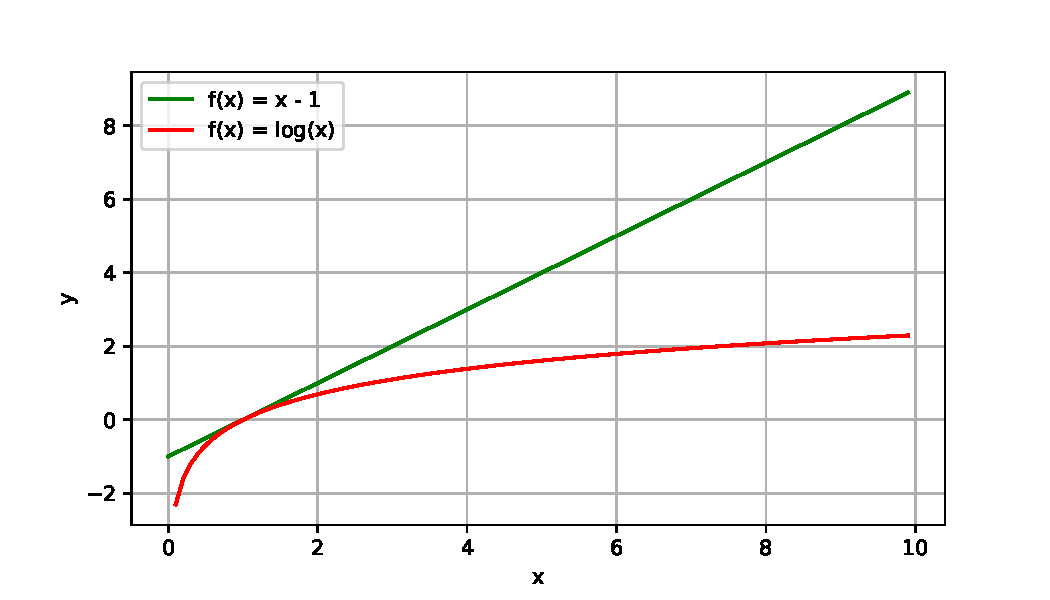
\includegraphics[width=\textwidth]{log_vs_lin.pdf}
 \caption{}
 \label{fig:log_vs_lin}
 \end{figure}
 
 Today I would like to neaten up my understanding of the EM algorithm, build a factor analyzer, and read the first chapter of Boyd's \emph{Convex Optimization}.
 
 \experiment{Fulbright Scholarship}
 Fulbright scholarships are awarded by the US Bureau of Educational and Cultural affairs under the Department of State. Approximately 800 scholarships are awarded each year to international students (Visiting Scholars). Emphazises leadership, commitment to international engagement, and cultural interaction. Fulbrighters seek to create a more peaceful and prosperous world. Funding is available for research and/or lecturing.
 
 Benefits of studying in the USA:
 \begin{itemize}
 	\item Quality of research
 	\item Flexible and interdisciplinary
 	\item International experience
 	\item Funding
 \end{itemize}
 
Fulbright postgraduate scholarships (http://www.fulbright.org.uk/going-to-the-usa/postgraduate): any master's/doctoral degress at any graduate programme at a US university. The scholarship offers:
\begin{itemize}
	\item Financial contributions towards the first year of study
	\item Sickness and accident coverage
	\item J-1 visa sponsorship and pre-departure orientation
	\item Support whilst in the USA
	\item Access to the Fulbright alumni network
\end{itemize}
  The programme aims to foster cultural understanding between the US and UK - little previous experience with the USA is desirable.
Awards available:
\begin{itemize}
	\item Brown University: PhD in any discipline.
	\item The New School: Master's degree in any discipline.
	\item Lloyd's of London: Master's degree in any discipline related to risk.
	\item University of South Florida: PhD in any discipline.
	\item Fulbright: Master's/PhD/research at any university.
	\item Elsevier Data Analytics: Postgraduate study requiring data analysis or research at any university.
\end{itemize}
  ``We are looking for applicants who can engage with the USA in an atmosphere of openness, academic integrity and intellectual freedom, thereby promoting mutual understanding.''
Desirable applicants would be able to demonstrate:
\begin{itemize}
	\item Strong academic proposals and/or research projects
	\item Ambassadorial skills
	\item Intercultural sensitivity
	\item Genuine desire to learn aspects of American culture
	\item Extracurricular activities
	\item Community involvement
	\item Leadership potential
	\item Plans to further the Fulbright mission and give back to the UK upon returning
\end{itemize}

Applications process:
\begin{enumerate}
	\item Read the UK-specific instructions.
	\item Applications open: link on the bottom of this page (http://www.fulbright.org.uk/going-to-the-usa/postgraduate/fulbright-postgraduate-scholarships/how-to-apply). This requires bio information, academic/professional accomplishments, Fulbright project plans, personal statement, details of the US institutions that you intend to apply to, and three reference nominations.
	\item Upload the US-UK Fulbright Commission Form to this applications.
	\item Upload other information (passport, CV, transcripts, US university admission letter, portfolio)
\end{enumerate}
Applications to US universities must be made separately and in good time. If shortlisted, the interview will be in January or February. Status is notified in March. Applications open in August. The British Fulbright Commission provide lots of information regarding American University's application procedures (see here: http://www.fulbright.org.uk/going-to-the-usa/postgraduate/educationusa-advice).
  
 
\experiment{VEST Scholarship}
The Charles M. Vest NAE Grand Challenges for Engineering International Scholarship Program provides an opportunity for graduate students at international universities to pursue reserach addressing a global Grand Challenge at leading United States university. The goals of the Vest Scholarships are to provide a platform to exchange ideas, share problem-solving skills and strengthen international  relationships in order to advance progress in some of the most critical global challenges in the twenty-first century. The scholarship offers;
\begin{itemize}
	\item The opportunity to spend a year at a leading US engineering school pursuing research.
	\item Living and travel expenses and tuition covered by the host institution for the 12-month duration of the scholarship.
	\item An opportuntiy to perform research in the laboratory of a leading faculty scholar.
	\item Access to engineering classes and academic credit towards graduate degrees.
	\item 10 scholarships available - one at each partner institution.
\end{itemize}
Applicants must be enrolled in a graduate-level engineering program at the time of application and during the scholarship year. Applicants will be asked to submit a personal statement proposing a one-year research and study plan that addresses one of the 14 Grand Challenges for Engineering. Winning statements will be those that presen the most compelling and potentially impactful proposal, and that map best onto Grand Challenge activities at the participating institutions. Academic aptitude and potential for success will be an important part of the selection process. Applications open August 1 and close November 1. The winnders are contacted on February 15, 2018.

The Grand Challenges relevant to me are:
\begin{itemize}
\item Engineer the tools of scientific discovery (Caltech, Duke, Washington)
\item Advance health informatics (MIT, North Carolina, University of Minnesota)
\item Advance personalized learning (MIT, Olin)
\end{itemize}
It is only possible to apply under one Challenge. Read more about each challenge and institution at \texttt{https://vestscholars.org/research-challenges}.



\labday{Sunday, 25th June 2017}
(08:45 - 09:45) I overslept this morning (it's a Sunday), but I can pick up the hours this afternoon/evening. Yesterday I built part of a factor analyzer, produced detailed notes on the EM algorithm - namely a proof for the bound used and a proof for the choice of density function in the E-step - and read about the Fulbright and Vest scholarships.

Today I would like to:
\begin{itemize}
	\item Finish the factor analyzer
	\item Email MM and ET with a review of what I've been up to this week:
	\begin{itemize}
		\item Reading: generative models of data using hidden variables and the EM algorithm (esp. mixture of gaussians and factor analyzers). Built a univariate MoG model and a factor analyzer for face identification. Read Canny \emph{A Computational Approach to Edge Detection}. Read paper \emph{Detection and classification of surface defects of gun barrels using computer vision and machine learning}. I started a MOOC focused on convex optimization.
		\item DNV: IT induction. Gained access to wind turbine and PV panel datasets. Began work on PV panel problem to detect cracked panels. I built several simple classifiers (a random forest, a boosted forest, and a radial basis SVM) against a subset of the data.
		\item NW Reading: Bayesian linear, nonlinear, and sparse linear regression models (2 days). Bayesian logistic, nonlinear logistic, and boosting models (2 days). Graphical models (2 days).
		\item NW DNV: If Azure access is available, train a convnet against the solar panel dataset. Set up a dummy generative adversarial model for synthetic data generation.
	\end{itemize}
	\item Read the GAN paper.
	\item Fix the size of the augmented dataset. Change the programme such that it augments both cracked and non-cracked panels (add Bernoulli variable to speckling).
	\item Build a HOG feature generator.
	\item What's SIFT?
	\item Use \texttt{skimage}'s tools to segment the panels.
	\item Email family describing what you've been up to this week.
\end{itemize}

There are 7 weeks left as of right now:
\begin{itemize}
	\item Week 2:
		\begin{itemize}
			\item Read five papers. (9 hours)
			\item Complete two sets of lectures from \emph{Convex Optimization} (12.5 hours).
			\item Complete Chapters 8, 9, 10 of \emph{Computer Vision} (25 hours).
			\item Complete as much of the TensorFlow Udacity course as you can. (25 hours).
			\item Complete and report the PV panel crack detection problem (12.5 hours).
			\item 
		\end{itemize}
	\item Week 3:
		\begin{itemize}
			\item Read five papers. (9 hours)
			\item Complete two sets of lectures from \emph{Convex Optimization} (12.5 hours).
			\item Complete Chapters 11, 12, 13 of \emph{Computer Vision} (25 hours).
			\item Finish the TensorFlow Udacity course. (25 hours).
			\item Choose a research problem to solve.
			\item Complete and report the PV panel crack detection problem (12.5 hours).
		\end{itemize}
	\item Week 4:
		\begin{itemize}
			\item Read five papers. (9 hours)
			\item Complete two sets of lectures from \emph{Convex Optimization} (12.5 hours).
			\item Complete Chapters 14, 15, 16 of \emph{Computer Vision} (25 hours).
			\item Work on the research problem (37.5 hours).
			\item Set a reminder to register for NIPS.
			\item Set a reminder to start investigating postgraduate degrees at universities (and schedule submission dates, exams and so on).
		\end{itemize}
	\item Week 5:
		\begin{itemize}
			\item TBD
		\end{itemize}
\end{itemize}

(12:30 -14:00 ) Reviewed yesterday's work, made notes on the applications of the models discussed in Ch.7 of \emph{Computer Vision}. These included regression onto missing data (described in the context of reorienting faces), using t-distributions to model patches of images for object classification, identifying faces using factor analysis, and understanding transformations as hidden variables.

(14:00 - 16:25) Building factor analyzer for face recognition (likelihood fitter)

(18:00 - 21:00) Fixed the fitting part of the factor analyzer (yay)

Hours worked this week:
\begin{itemize}
	\item Monday: Untracked.
	\item Tuesday: Untracked.
	\item Wednesday: 8.5hrs
	\item Thursday: 11hrs
	\item Friday: 7.75hrs
	\item Saturday: 7hrs
	\item Sunday: 8hrs
\end{itemize}

\experiment{Prince, \emph{Computer Vision} (Ch. 7, Modeling Complex Data Densities}
 Yesterday I finished this chapter by re-covering factor analyzers - generative models that use a subspace to quantify covariance rather than the full feature space - and tying up the loose ends in my understanding of the EM algorithm. The particular loose ends covered were:
 \begin{itemize}
 	\item Proof that the bondary function is less than the log-likelihood. That is, we proved that:
 	\[
 		\sum_{i=1}^I \int q_i(h_i) \log\Bigg[\frac{\text{Pr}(h_i, x_i| \theta)}{q_i(h_i)} \Bigg]dh_i \ \leq \ \sum_{i=1}^I \log\Bigg[\int q_i(h_i) \frac{\text{Pr}(h_i, x_i| \theta)}{q_i(h_i)}dh_i \Bigg]
 	\]
 	Or, in a form that gives a better insight into what's actually going on:
 	\[
 		\sum_{i=1}^I E\Bigg[\log\Big[\frac{\text{Pr}(x_i, h_i|\theta)}{q_i(h_i)}\Big]\Bigg] \leq \sum_{i=1}^I \log\Bigg[E\Big[\frac{\text{Pr}(x_i, h_i|\theta}{q_i (h_i)}\Big]\Bigg]
 	\]
 	The proof for this inequality relies on Jensen's inequality, which states that:
 	\[
 		E[\log y] \leq \log[Ey]
 	\]
 	I haven't proven this, but logarithms tend to squish big numbers, hence shrinking their expectations. I think it's the case that this form of boundary is chosen because it makes it clearer what the the appropriate density functions $q_i(h_i)$ to maximize the boundary are.
 	\item In particular, we proved that the choice of $q_i(h_i)$ in the E-step should be the hidden variable's posterior given the data and parameters at that step:
 	\[
 		\hat{q}_i(h_i) = \text{Pr}(h_i | x_i, \theta^{[t]})
 	\]
 	We did this by rearranging the optimization problem of the E-step to bring out the Kullback-Leibler divergence:
 	\[
 		q_i(h_i) \cdot \log\Big[\frac{\text{Pr}(h_i|x_i, \theta)}{q_i(h_i)}\Big]
 	\]
 	which can be shown to always be negative, further meaning that the boundary-maximizing choice of $q_i(h_i)$ is indeed the aforementioned posterior.
 	\item On a high level, I understood why the boundary function is always less than or equal to the log-likelihood of the joint distribution of $\text{Pr}(x_i, h_i|\theta)$, and what choice of $q_i(h_i)$ satisfies the equality of the two for a given choice of model parameters $\theta$. The EM algorithm is useful because it allows nonlinear functions to be optimized, provided that they can be expressed in terms of a hidden variable.
 \end{itemize}
 After making notes on this, I started building a factor analyzer to identify faces from images. I wrote out the source code; today I intend to create a functional programme. I think I'll also go through the applications, since these are what have really been allowing me to convert theoretical knowledge to practical utility.
 
 Idea: regressing cracks onto the rest of their panels, then conditioning over an incomplete uncracked panel to generate a cracked panel image (See pp. 104 of \emph{Computer Vision}).
 
 I think I would benefit most from Chapter 7's problems if I were to do them in the middle of next week (say Thursday) rather than right now.
 
  \experiment{Prince, \emph{Computer Vision} (Ch. 8, Regression models}
 \begin{figure}[h!]
 \centering
 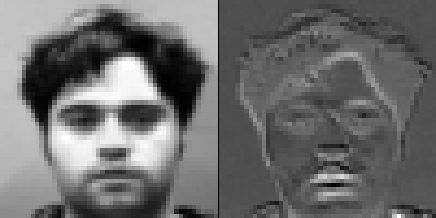
\includegraphics[width=0.5\textwidth]{factor_analyzer_class_mean_and_factor.png}
 \caption{The mean (left) and single factor (right) of a grayscale image from the factor analyzer.}
 \end{figure}
 
 
 
 \labday{Monday, 26th June 2017}
 
 \experiment{Summary}
 (08:00 - 11:00) Prince's \emph{Computer Vision}, Ch. 8. Linear regression, Bayesian linear regression, nonlinear regression (inc. kernels, radial basis functions, and gaussian process regression), sparse linear regression.
 
 (11:15 - 13:00) Tensorflow lectures - received first assignment.
 
 (15:15 - 16:45) Sent a weekly update to ET and MM. It was as follows:
 \begin{displayquote}
 \small
 Hello Professor Mirmehdi,\\[1em]
I hope you're well. Paul Harper introduced us several months ago: I'm an undergraduate researcher in machine vision working at the University/DNV-GL. Pleased to meet you (again).\\[0.7em]
My reason for emailing is that since you are my point of contact with the University and are an expert in machine vision, I thought it would be a good idea if gave you a weekly update of what I've been up to. This is so that:
\begin{itemize}
\item[(a)] you know I'm spending my placement time productively
\item[(b)] I can benefit from your guidance as to whether I'm following an unpromising path / could make use of some theory/tools in particular.
\end{itemize}
I appreciate that you are busy and will try to keep these emails succinct - if you'd rather not hear from me, please let me know. Anyway, last week I:
\begin{itemize}
\item Spent a lot of time reading about how to use the expectation maximisation algorithm. I built a factor analyser to identify faces in this dataset (http://cswww.essex.ac.uk/mv/allfaces/index.html) and a Gaussian mixture model against another dataset. I know that these are quite old-school methods, but I think understanding them will aid my general grasp of machine learning and vision.
\item Began working on classifying grayscale images of cracked PV panels for DNV. I've cleaned, subset, augmented and split a dataset that was originally of about 50 unique panels. I also ran a random forest and a radial basis function support vector machine against the training set, without any preprocessing (apart from standardisation). I was planning to use a histogram of oriented gradients as the classifier's input (possibly in addition to the pixel intensities?). This is because the cracks seem to be distinguished by their orientation. I may try a convnet, but think it will probably overfit.
\item Started a course on numerical methods for convex optimisation. This is in an effort to understand how to phrase optimisation problems in a sensible way. I think the first few weeks focus on theory, after which there's a strong emphasis on applications.
\item Became more interested in methods for generating synthetic data. I was thinking of building a generative adversarial network (GAN, a pair of competing neural networks, one of which attempts to generate fake images, the other which tries to spot images that are fake) and looking at using generative models of cracked PV panels to transplant fake cracks onto images of uncracked panels
\end{itemize}
This week I was going to finish the PV panel classifier and summarise its performance in a report. I have also allocated a big chunk of time to reading, some of which will go towards reading about and building GANs.\\[0.7em]
Do you have time to meet this week? I was had a few questions about choice of model and preprocessing procedure for the PV panel classification task. Also, your suggestions of what I should read about/work on to make the placement worthwhile would be really useful to me.\\[0.7em]
Thank you and have a great week,\\[0.7em]
Jerome
\end{displayquote}
 
 (16:45 - 17:45) Tensorflow assignment.

 (17:55 - 18:40) Read Ch. 1 of \emph{Convex optimization}. The course begins by focusing on the maths of convex sets, functions, and optimization, before moving onto applications and algorithms. A convex function is a function that is less than or equal to a line between two points in its 
 
 (18:45 - 19:45) Finished the Tensorflow assignment. It focused on data cleaning and fitting a logistic regression classifier. It didn't actually involve using TF! I used the package \texttt{tqmd}, which made it easy to associate loading bars with \texttt{for} loops. My memory of pickling was also refreshed - it is a pretty convenient way to store large Python structures on disk for access at short notice.
 
 \experiment{Prince, \emph{Computer Vision} (Ch. 8, Regression models)}
 After the previous chapter's focus on various generative models, which modeled the data's distribution for given world states, this chapter focuses on discriminative methods for regression. It began by introducing a simple linear model for a univariate continuous world state $w$ and continuous multivariate vector $\mathbf{x}$:
 \[
 	\text{Pr}(\mathbf{w}|\mathbf{X}, \phi) = \text{Norm}_w[\mathbf{X}^T \phi, \sigma^2]
 \]
 Where $\mathbf{X}$ is a $D \times I$ matrix of $I$ examples, each of $D$ dimensions. In other words, we assume that the mean response is a linear function of the inputs $\mathbf{x}$, with constant variance. The model's parameters can be fit using maximum likelihood, maximum a posteriori, or bayesian analysis. The ML estimate of the parameters is:
 \begin{gather*}
 	\phi = (\mathbf{X}\mathbf{X}^T)^{-1}\mathbf{X}^T \mathbf{w}\\[1em]
 	\sigma^2 = \frac{(\mathbf{w} - \mathbf{X}^T\phi)^T(\mathbf{w} - \mathbf{X}^T\phi)}{I} 
 \end{gather*}
Notice that here the likelihood being maximized is $\text{Pr}(w|x, \theta)$, whereas when fitting the generative methods we maximized the likelihood $\text{Pr}(x|w, \theta)$.

Several flaws in the simple linear model were pointed out:
\begin{itemize}
	\item There is no embedded representation of the uncertainty associated with extrapolation - the model is as confident where there have been many observations as it is where there are none.
	\item A linear function may not be representative of the true relationship between the inputs and mean response.
	\item Many of the input features may be redundant or of little predictive power, but will be assigned tiny coefficients upon fitting the model - this makes the model needlessly complex.
\end{itemize}
To represent the uncertainty in the model's coefficients more accurately, we can model the parameters as normally distributed variables:
\[
	\text{Pr}(\phi) = \text{Norm}_{\phi}[\mathbf{0}, \sigma_p^2]
\]
Where $\sigma_p^2$ is a hyperparameter (we'd usually fix it to a large value to represent our initial uncertainty). Then, when fitting the model, we can use Bayesian analysis rather than maximum likelihood:
\[
	\text{Pr}(\phi|\mathbf{X}, \mathbf{w}) = \frac{\text{Pr}(\mathbf{w}|\mathbf{X}, \phi)\cdot \text{Pr}(\phi)}{\text{Pr}(\mathbf{w}|\mathbf{X})}
\]
This yields a normal posterior distribution over the parameter values with a covariance that increases with $\mathbf{x}$. To make predictions using this distribution, compute the posterior predictive and evaluate its value at the query world state and data.

Several matrix identities were introduced in this section with the intention of making matrix inverse calculations less expensive. One of these was the Sherman-Morrison-Woodbury identity, which can be used to speed up posterior and posterior predictive inference in the aforementioned Bayesian model.

To work around the issue that the expected response and the inputs are unlikely to have a linear relationship, the model was generalized to nonlinear functions in neat way: simply replace the raw input vector $\mathbf{x}$ with its value under nonlinear transformation:
\[
	\mathbf{z} = \mathbf{f}[\mathbf{x}]
\]
Then model the relationship between the world state and input as a linear one:
\[
	\text{Pr}(\mathbf{w}|\mathbf{Z}, \phi) = \text{Norm}_{\mathbf{w}}(\mathbf{Z}^T\phi, \sigma^2)
\]
Apply the equivalent versions of the ML estimates or the Bayesian analysis methods mentioned earlier to determine the parameters, then evaluate this epression at a new query for inference. The parameters of the nonlinear functions can be defined beforehand, or they can be fit. To fit them, we need to marginalize the above equation over $\phi$:
\[
	\text{Pr}(\mathbf{w}|\mathbf{Z}) = \int \text{Pr}(\mathbf{w}|\mathbf{Z}, \phi)\cdot\text{Pr}(\mathbf{\phi})\cdot d\phi
\]
We can then maximize this - the evidence - again the nonlinear function's parameters $\mathbf{\lambda}$:
\[
	\hat{\mathbf{\lambda}} = \argmax_{\mathbf{\lambda}} [\text{Pr}(\mathbf{w}|\mathbf{Z})]
\]
Use a nonlinear optimization procedure (i.e. local search with multiple instantiations, global search) to solve this.

If $\mathbf{z}$ is very high-dimensional, we can replace the dot products $\mathbf{z}_i^T\mathbf{z}_j$ in the ML and Bayesian models with the kernel function $k[\mathbf{x}_i, \mathbf{x}_j]$. 

The final area that I began to work on was sparse linear regression, which pushes coefficient values towards zero. By using prior distributions that favour zero-valued coefficients, it's possible to do exactly this.


 \labday{Tuesday, 27th June 2017}
 Today I would like to:
 \begin{itemize}
 	\item Summarize yesterday's work
 	\item Finish the Ch. 8 of \emph{Computer Vision} (2 hours)
 	\item Build at least one of the regression models described in this chapter (2 hours)
 	\item Spend two hours on the Tensorflow lectures (2 hours)
 	\item Spend four hours on the PV panel classifier: (4 hours)
 	\begin{itemize}
 		\item Fix the augmenter balance.
 		\item Augment undamaged panels.
 		\item Build a gradient descriptor.
 		\item Document progress so far.
 	\end{itemize}
 	\item Print and read GAN papers
 \end{itemize}
 
 \experiment{Summary}
 (07:00 - 08:00) Summarized yesterday's work.
 (08:00 - 11:00) Sparse regression, dual linear regression. 
 
 Dual linear regression expresses the gradient vector in terms of the training data points. It's appropriate for situations in which the data has many more dimensions than examples.
 
  Sparse linear regression places a t-distributed prior on each of the gradient values to represent the fact that many of the gradient elements may not be useful in predicting the response. To fit the mean and variance of the parameter vector of the sparse regression model, it is necessary to maximize an approximation of the likelihood function. To make this approximation, a function must be maximized with respect to the hidden variables of the t-distributions. In reality, the likelihood function and the parameters that maximize it are optimized simultaneously.
 
  Relevance vector regression combines the principles of sparse and dual linear regression to produce an efficient regressor: a prior is placed on each element of the dual vector (which correspond to weightings of each observation) that pushes it towards zero, then the mean and variance of this dual vector's posterior is computed while simultaneously approximating the likelihood function by maximizing a function w.r.t. the t-distribution's hidden variables. Relevance vector machines describe predictive models to be described in terms of just a few datapoints, as opposed to attempting to weight high-dimensional input vectors or use all of the datapoints available (which makes optimization expensive).

(11:00 - 13:00) Swept the steps. Took Lunch.

(13:00 -14:00) Bio for The Bakery.

(14:00 - 15:00) More on sparse linear regression. I've found it quite difficult to grasp, and still feel as though I'm missing something. Say we have a linear model:
\[
	\text{Pr}(w|X, \sigma^2, \phi) = \text{Normal}_{w}[X^T\phi, \sigma^2 I]
\]
$X$ is a $D \times I$ matrix of inputs, $\sigma^2$ is common variance, $w$ is a vector of $I$ responses. A non-sparse Bayesian linear model would assume a normal prior distribution $\text{Norm}_\phi[\mathbf{0}, \sigma_p^2]$ over the weights, where $\sigma_p^2$ is large. In combination with the normal likelihood above, this would yield a normal posterior distribution:
\[
	\text{Pr}(\phi|w, X, \sigma^2) = \frac{\text{Pr}(w|X, \phi, \sigma^2)\cdot\text{Pr}(\phi)}{\text{Pr}(w|X, \sigma^2)}
\]
Since the posterior and the likelihood were normal, the posterior predictive had a closed-form solution (yet another normal distribution). It was also possible to compute the posterior directly.

In a sparse linear model, the prior term is adjusted to weight zero-valued elements of $\phi$ more heavily. The purpose of this is to identify input that have little predictive value. This is achieved using a multivariate $t$-distribution:
\[
	\text{Pr}(\phi) = \prod_{d = 1}^{D} \text{Stud}_{\phi_d}[0, 1, \nu]
\]
Problematically, this means that there is no analytical expression for the posterior distribution over the weights $\phi$. We still need an expression for this posterior, however, to be able to express the posterior predictive distribution. The book asserts that we can estimate the parameters $\mu$, $\Sigma$ of a normal distribution that approximates the weight's true posterior by maximizing an approximation to the model's evidence, $\text{Pr}(w|X, \sigma^2)$, with respect to the t-distribution's hidden variables and the model's common variance $\sigma^2$. I am puzzled about:
\begin{itemize}
	\item[(a)] Where the normal posterior came from to approximate the product of a normal and t-distribution.
	\item[(b)] How the values for the hidden variables influence the choice of weights.
\end{itemize}
The former point I think I can appreciate in an unrigorous sense, but the latter needs more thought. The hidden variables of the t-distribution affects the distribution's variance - smaller values of $h_d$ suggest a larger variance, further implying a more probable non-zero value for $\phi_d$. So the idea with solving for values of the hidden variables is to stretch the prior in the directions that are likely to have non-zero values. By contrast, $\sigma^2$ has to be updated alongside the hidden variables because when the uncertainty in the values of the hidden variables changes, so too will the uncertainty in the response. I think I'm getting closer with this - maybe a few more readings...

(15:00 - 16:15) Wrote the above on sparse regression. Replied to John Ryan.

(16:15 - 17:50) Built a dual regression model on Iris dataset.
\begin{figure}[h!]
\centering
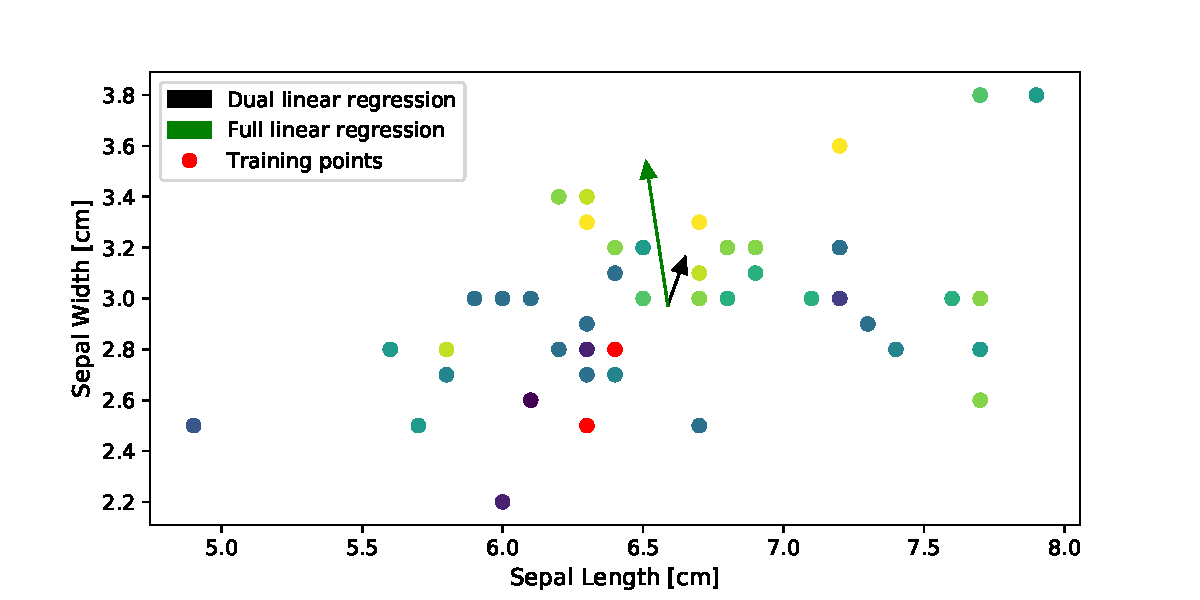
\includegraphics[width=0.8\textwidth]{dual_linear_regression.pdf}
\end{figure}

(17:50 - 19:45) Built a Gaussian nonlinear regression model.
\begin{figure}[h!]
\centering
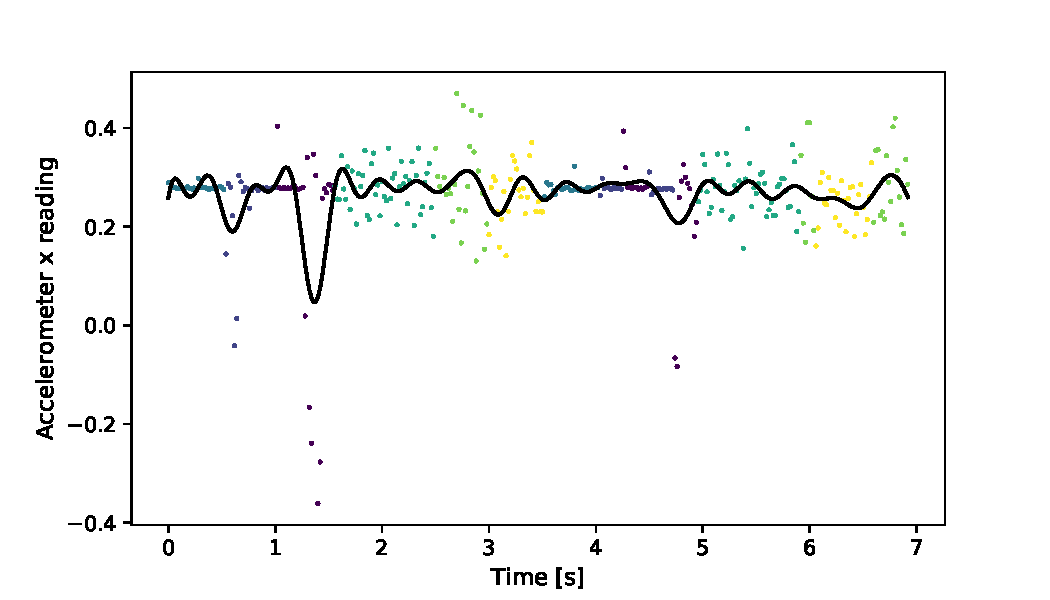
\includegraphics[width=0.8\textwidth]{nonlinear_regression.pdf}
\end{figure}



labday{Wednesday, 28th June 2017}
Yesterday I built a nonlinear regression model and a dual linear regression model. 

The nonlinear model has a simple premise - perform a nonlinear transformation of the inputs, then perform a linear regression of the transformed inputs onto the response. Kernels can be used to make this process much more efficient/feasible.

The dual model assumes that the gradient vector is in the subspace described by the observations. It's useful when the dimensionality of the data exceeds the number of observations. In such a situation, linear regression is not possible since its model would be under-constrained. Why is it valid to assume that the gradient vector lies in the subspace described by the observations? In short, the assumption is justified by the observation that if input variation is not observed in a given direction, then there is no information available that can be used to compute a gradient in that direction.


(09:30 - 12:30) \emph{Convex Optimization} Lecture 2 - convex sets.

(13:45 - 17:30) Tensorflow work. Moved from the logistic regression model to neural networks by introducing nonlinear transfer functions (specifically, RELUs). Built a two-layer network for 10-way classification. Understood the TensorFlow workflow: set up a graph, pass the graph to a session. Reviewed stochastic and minibatch gradient descent, momentum (taking a running average of the loss gradient and using it to choose the direction of optimization for the current iteration), l2 regularization (penalizing  large weights - why?), dropout (to encourage redundancy in the network), learning rate decay (to permit better overall convergence), and early termination (to avoid overfitting).


(19:00 - 21:15) Prince, \emph{Computer Vision} (Ch. 9, Classification models). Logistic regression, Newton's method for making an ML fit of its parameters. Laplace approximation for a distribution. Integrating a multivariate normal distribution over one dimension instead of many via a linear projection. Highlighted the weaknesses of logistic regression:
\begin{itemize}
\item Using maximum likelihood to fit the parameters whitewashes the actual uncertainty in a class prediction (resolved via Bayesian logistic regression).
\item Linear decision boundaries are sometimes inadequate.
\item The model is expensive to fit in many dimensions, and is prone to overfitting in wide situations.
\end{itemize}

\experiment{Boyd, \emph{Convex Optimisation} (Lecture 2)}
The lecture covered various basic types of convex sets, and operations that preserve convexity. Simple convex sets that he brought up included:
\begin{itemize}
	\item The basic convex set: $S : \{x_1, x_2|\theta x_1 + (1 - \theta)x_2 \in S, \theta \in [0, 1]\}$
	\item Affine sets: $\{x | \theta x_1 + (1 - \theta)x_2, \theta \in \mathbb{R}\}$
	\item Hyperplanes: constraints on single elements from an affine set; $\{x | a^t x = b, a \in \mathbb{R}^n, b \in \mathbb{R}\}$
	\item Convex hulls: the set of all convex combinations of points in a set: $x = \theta_1 x_1 + ... + \theta_k x_k$ with $\sum \theta = 1, \theta_i \geq 0 \ \forall \ i$.
	\item Halfspaces: like a hyperplane, but with an inequality. $\{x | a^T x \leq b\}$.
	\item Convex cones: any linear combination of two points, provided that the coefficients are positive. $C : \{x|x = \theta_1 x_1 + \theta_2 x_2, \quad \theta_1, \theta_2 \geq 0\}$
	\item Euclidean balls and ellipsoids (linear transformations of a unit ball). $\{x | (x - x_c)P^{-1}(x - x_c) \leq 1\} = \{x_c + `	0Au | \|u\|_2 \leq 1\}$. A euclidean ball is the set of points that satisfy $\{x| \|x - x_c\|_2 \leq r\}$. We also defined a norm as a function that satisfies various conditions.
	\item Polyhedra: A set of points satisfying finitely many inequalities (halfspaces) and equalities (hyperplanes). $\{x|Ax \preceq b, Cx = d\}$.
\end{itemize}
He emphasized that these basic convex sets in combination with convexity-preserving operations are useful for demonstrating a set's convexity. Alternatively, we can use the basic definition of convexity to show that a set is convex.

The second half of the lecture focused on these convexity-preserving operations, which were the:
\begin{itemize}
	\item Intersection
	\item Affine function
	\item Perspective function - the division of the first $n$ elements in a vector by the vector's $n$th and final element.
	\[
		P(x, t) = \frac{x}{t}, \quad \text{dom}P = \{(x, t)|t > 0\}
	\]
	\item Linear-fractional function - the perspective function after an affine transformation.
	\[
		f(x) = \frac{Ax + b}{c^T x + d}, \quad \text{dom}f = \{x|c^T x + d > 0\}
	\]
\end{itemize}



\labday{Thursday, 29th June 2016}

(07:10 - 12:50) PV panel classifier work

(14:00 - 15:20)(16:45 - 18:45) Computer Vision exercises (Ch. 5, ). Distribution of a multivariate normal r.v. under an affine transformation. Marginalizing a normal distribution using an affine transform. Standardizing a multivariate normal distribution. Proving the Schur complement identity. (Up to 5.5) (1, 2, 3, 4, 7, 8).

(18:45 - 20:45) Computer Vision exercises (Ch. 7) Describing generative models for a continuous input vector and a binary response. Described how the t-distribution can be used to make this type of model robust to outliers (e.g. mislabelled samples). Derived the component weight updates in the M-step of the EM algorithm when fitting a Gaussian mixture model. Learnt how to use Lagrange multipliers to solve constrained optimization problems (tangency between the constraint and objective function gradients!). 



\labday{Friday, 30th June 2016}
(09:00 - 11:00) Solving problems from Ch. 8 of \emph{Computer Vision}. Deriving the t-distribution from the gamma and normal distributions. Deriving the M-step values for the mean and covariance values in a Gaussian mixture model.
(11:00 - 13:00) Nonlinear logistic regression - as with linear regression, we simply apply the nonlinear transformation to the inputs. Fitting the model requires a nonlinear optimization method - fitting these models is usually done using maximum likelihood, since prior modeling over both the gradient vector $\phi$ and the parameters of the nonlinear function requires a lot of effort.

 I also made notes on the dual logistic regression classifier, and how it can be fit using either maximum likelihood orBayesian inference. The latter requires the Laplace approximation - approximating a distribution using a normal distribution with equal mean and second derivative at the mean to the actual distribution being modeled. Fitting logistic regression or dual logistic regression models in a Bayesian manner requires that the true parameter ($\phi$ or $\varphi$) posterior distribution's parameters be approximated by their equivalents in the maximum a posteriori fit.

 This afternoon I intend to:
 \begin{itemize}
 	\item Finish Ch. 9 of \emph{Computer Vision}
 	\item Build the Generative Adversarial Network described by Analytics Vidyha
 	\item Build a kernelized dual logistic regression classifier.
 	\item Finish the \emph{Convex Optimization} lecture.
 	\item Find papers relating to crack detection.
 	\item Complete IET end-of-year assessment.
\end{itemize}

 
 (14:40 - 18:40) Chapter 8 of \emph{Computer Vision}. A lot of material was covered:
 \begin{itemize}
 	\item Nonlinear logistic regression
	\item Dual logistic regression
	\item Kernelized Bayesian nonlinear dual logistic regression (a.k.a. Gaussian process classification)
	\item Relevance vector classifiers (sparse Gaussian process classifiers)
	\item Forward stepwise selection
	\item Boosting
	\item Classification trees/gating functions
	\item Multiclass logistic regression
\end{itemize}
I should definitely type up a review of these areas - if not this evening, then tomorrow.

(18:40 - 20:05) Labelled images (annotations, not y/n).

(20:05 - 20:45) Resized, masked images.

\experiment{Meeting with MM}
Topics of conversation:
\begin{itemize}
	\item PV panel classification problem : identifying cracks in scans of PV panels.
	\item Questions:
	\begin{itemize}
		\item Very small dataset problem: 50:50 train/test, split the training data 70:30 into training/validation sets (i.e. I have very poor resolution on what the generalization error of the models I'm fitting is likely to be).
		\item What preprocessing can I use to enhance the cracks?
			\begin{itemize}
				\item The images have been equalized, resized for intensity classification.
				\item Augmented the training images to expand the dataset size.
				\item Did not augment testing images.
				\item I've used HOGs, which resulted in improved performance (with more data, I think this would be a viable solution).
				\item Other edge/feature detectors?
				\item Possible idea: Cluster panels according to model, subtract an undamaged panel from the input?
			\end{itemize}
		\item Are there any papers that he would recommend?
		\item Other methods for expanding the amount of data available?
	\item Wind turbines:
		\begin{itemize}
			\item Meeting the inspections team next week
			\item ET wants me to focus on using visible spectrum data
			\item Use stills, as opposed to sequenced videos
			\item Need to label the data - recommendations on how to do this?
			\item I will email him images of the turbines
		\end{itemize}
	\item General placement enquiries:
		\begin{itemize}
			\item What can I do that would be useful/what problems would be tractable for the placement, but would still be interesting/novel?
			\item Does he think that doing an (admittedly small) piece of original research is possible in this timeframe?
			\item I'm interested in synthetic data generation - does this sound like a suitable area to focus my efforts?
		\end{itemize}
	\end{itemize}
\end{itemize}


\labday{Monday, 3rd July 2017}
(06:30 - 11:10) PV Panel subsetter -...

(11:30 - 12:10) Meeting with MM. Notes:
\begin{itemize}
	\item Local binary patterns
	\item Gabor filters
	\item 
\end{itemize}

(12:45 - 13:15) Lunch with Paul Harper.

(13:45 - 18:00) DNV.

(21:00 - 22:00) TF Reg. assignment.


\labday{Tuesday, 4th July 2017}
(07:30 - 11:00) Finished Tensorflow assigment. Emailed Mikkel Skou requesting Azure access.
(11:30 - 12:00) Skype call with ET and RD w.r.t. Azure access. Learnt how to save/restore sessions in TensorFlow.
(12:15 - 13:15) Conceived of probabilistic relaxation method. Figuring out details.
(13:45 - 15:00) Meeting with James and ET at DNV w.r.t. image processing. They recommend vastly expanding the feature space, possibly focusing on cracks located at the edges.
(15:00 - 22:00) Meeting family. No work.



\labday{Wednesday, 5th July 2017}
Today I plan to:
\begin{itemize}
	\item Build the probabilistic relaxation model.
	\item Generate at least ten sets of candidate extracted features.
	\item Build and report on the progress with the PV panel classification problem so far.
	\item Read at least two papers.
	\item Finish \emph{Convex Optimisation} lecture 2.
	\item Understand the singular value decomposition.
	\item Summarize last weeks work (or lack thereof!)
\end{itemize}
Stay hungry, stay foolish.

(06:20 - 19:15) Built a generative normal model of crack/uncracked pixels. Fit a random forest to the resulting probabilities. Built lots of filters.
(19:15 - 20:30) Printed three papers at the University - Hough transform, probabilistic relaxation, and hidden markov models for crack detection.
(20:30 - 22:30) Read the Hough transform paper. Will summarize tomorrow when I wake up.


\labday{Thursday, 6th July 2017}
Good morning - it's 06:50. Yesterday I experimented with various convolutional filters, some of which were moderately successful. I also read a paper on the Hough (`how') transform, \emph{Use of the Hough Transformation to Detect Lines and Curves in Pictures} by Ruchard Duda and Peter Hart. The Hough transform is used to detect colinear points in an image.

\experiment{\emph{Use of the Hough Transform to Detect Lines and Curves in Pictures}}
 The idea of the Hough transform is to map a point at $(x, y)$ in the figure domain onto a plane parameterized by $(\rho, \theta)$. $\theta$ corresponds to the angle between the plane and the origin and $\rho$ is the distance of the plane from said origin. The unit normal vector of the plane is $[\cos\theta, \sin\theta]$, such that the points $(x, y)$ are projected onto a line at an angle $\theta$ to the origin by:
\[
	\rho = x\cos\theta + y\sin\theta 
\]
. If $\theta$ and are $\rho$ are chosen correctly, then a colinear set of points in the figure will be projected onto a single point in the $\rho-\theta$ plane. In this way then, $\rho$ encodes the detected line's distance from the origin and $\theta$ the angle it makes with the $y$-axis. For the implementation:
\begin{enumerate}
\item Binarize the image.
\item Create a matrix with rows indexed by quantized values of  $\rho \in [0, R]$ and columns indexed by quantized values $\theta \in [0, \pi)$.
\item Project the points onto a vector that makes an angle $\theta \in [0, \pi)$ with the origin, then count the number of projected points that lie in each radial interval. Record this number in the matrix cells corresponding to the given angle and radial intervals.
\item Repeat (3) for all angles. The sum of each column will be equal to the total number of points.
\item Cells that have an unusually high number of points will tend to correspond to lines in the image.
\end{enumerate}
The Hough transform comes with a few warnings attached - high-scoring cells don't necessarily correspond to contiguous lines, the chosen resolution of cells has big implications for the method's efficacy, and careful thought needs to be given about the number of pixels in the lines of interest. The method can be generalized to other parameterizations beyond straight lines: All that's necessary is to parameterize a curve using the $x, y$ values. In general, points in $(x,y)$ on the geometry described by a function $f(\phi_1, ..., \phi_p)$ will map to single point in the space $\phi_1, ..., \phi_p$. By discretizing the values of $\phi$ and binning the positions of the points, it is possible to detect an arbitrary geometry. A parabola in $(x, y)$, for example, would be parameterized by:
\[
	(x - a)^2 + y^2 = b
\]



\end{document}
 